\section{Affine Varieties}

\begin{definition}
    Let $k$ be a perfect field. We define  \textbf{affine $n$-space} over $k$ to
    be the set
    \begin{equation*}
        \A^n(\bar{k})=\{P=(x_1, \dots, x_n) : x_i \in \bar{k}\}
    \end{equation*}
    where $\bar{k}$ is the algebraic closure of $k$. We define the set of all
     \textbf{$k$-rational points} of $\A^n$ to be
     \begin{equation*}
        \A^n(k)=\{P=(x_1, \dots, x_n) : x_i \in k\}
     \end{equation*}
\end{definition}

\begin{lemma}\label{1.1.1}
    Let $k$ be a perfect field, and $\bar{k}$ its algebraic closure. Then
    $\Gal{\faktor{\bar{k}}{k}}$ acts on $\A^n$ via the action
    \begin{equation*}
        P=(x_1, \dots, x_n) \xrightarrow{} \s{P}=(\s{x_1}, \dots, \s{x_n})
    \end{equation*}
    Moreover
    \begin{equation*}
        \A^n(k)=\{P \in \A^n : \s{P}=P \text{ for all } \s \in
        \Gal{\faktor{\bar{k}}{k}}\}
    \end{equation*}
\end{lemma}
\begin{proof}
    It is not hard to check that the action described above is indeed an action
    on $\A^n$. Moreover, since $\Gal{\faktor{\bar{k}}{k}}$ consists of all
    $k$-automorphisms  (i.e. automorphisms of $\bar{k}$ that fix $k$), then for
    any $\s \in \Gal{\faktor{\bar{k}}{k}}$, and $P \in k$, we have  $\s{P}=P$.
\end{proof}

\begin{definition}
    Let $k$ be a perfect field, and let $\af$ be an ideal of $\bar{k}[x_1,
    \dots, x_n]$. We define an \textbf{affine algebraic set} to be a set
    \begin{equation*}
        V_\af=\{P \in \A^n(\bar{k}) : f(P)=0 \text{ for all } f \in \af\}
    \end{equation*}
    That is, it is the set of all zeros of all polynomials in $\af$. We define
    the  \textbf{ideal} of $\V_\af$ to be the set
    \begin{equation*}
        I(V_\af)=\{f \in \bar{k}[x_1, \dots, x_n] : f(P)=0 \text{ for all } P
        \in V_\af\}
    \end{equation*}
\end{definition}

\begin{lemma}\label{1.1.2}
    Let $k$ be a perfect field, and $V$ an affine algebraic set. Then $I(V)$ is
    an ideal in $\bar{k}[x_1, \dots, x_n]$. Moreover, it is finitely generated.
\end{lemma}
\begin{proof}
    We have that $I(V)$ forms a subgroup of $\bar{k}[x_1, \dots, x_n]$, indeed,
    if $f,g \in I(V)$, then $-f \in I(V)$ and $g \in I(V)$. Moreover, if $g \in
    \bar{k}[x_1, \dots, x_n]$, then $gf \in I(V)$. Now, since $\bar{k}$ is a
    field, it is a PID, and hence Noetherian, so that by Hilbert's theorem (see
    \cite{atiyah-macdonald} or \cite{eisenbud}), $\bar{k}[x_1, \dots, x_n]$ is
    Noetherian, and so every ideal in $\bar{k}[x_1, \dots, x_n]$ must be finitely
    generated.
\end{proof}

\begin{lemma}\label{1.1.3}
    Let $V$ be an algebraic set over a perfect field, and consider the set
    $I(\faktor{V}{k})=I(V) \cap \bar{k}[x_1, \dots, x_n]$. Then $I(\faktor{V}{k})$
    is defined over $k$ if, and only if
    \begin{equation*}
        I(V)=I(\faktor{V}{k})\bar{k}[x_1, \dots, x_n]
    \end{equation*}
    Moreover, $I(\faktor{V}{k})$ is an ideal of $\bar{k}[x_1, \dots, x_n]$.
\end{lemma}
\begin{proof}
    Exercise
\end{proof}
\begin{corollary}
    If $V$ is defined over $k$ such that $I(\faktor{V}{k})=(f_1, \dots, f_m)$,
    where $f_1, \dots, f_m \in k$, then $V$ is the set of all solutions
    to the polynomial equations
    \begin{equation*}
        f_1(x_1, \dots, x_n)= \dots =f_m(x_1, \dots, x_n)=0 \text{ for all }
        x_1, \dots, x_n \in k
    \end{equation*}
\end{corollary}
\begin{corollary}
    If $V$ is defined over $k$, then the action of $\Gal{\faktor{\bar{k}}{k}}$
    on $\A^n$ induces an action on $V$, and
    \begin{equation*}
        V=\{P \in V : \s{P}=P \text{ for all } \s \in
        \Gal{\faktor{\bar{k}}{k}}\}
    \end{equation*}
\end{corollary}
\begin{proof}
    This result follows, in fact, immediately from lemma \ref{1.1.1}
\end{proof}

\begin{example}\label{example_1.1}
    \begin{enumerate}
        \item[(1)] Let $k$ be a perfect field and let $V$ the algebraic set in
            $\A^2$ given by the equation
            \begin{equation*}
                x^2-y^2=1
            \end{equation*}
            That is,
            \begin{equation*}
                V=\{P \in \A^2 : x^2-y^2-1=0\}
            \end{equation*}
            Suppose that $\Char{k} \neq 2$. Then $V$ is in 1--1 correspondence
            onto the set $\com{\A^2}{\{0\}}$ given by the map
            \begin{equation*}
                t \xrightarrow{} \Big{(} \frac{t^2+1}{2t},\frac{t^2-1}{2t} \Big{)}
            \end{equation*}
            That is, the set of all $k$-rational points, for  $\Char{k} \neq 0$
            of the set is given by
            \begin{equation*}
                \Big{(} \frac{t^2+1}{2t},\frac{t^2-1}{2t} \Big{)}
            \end{equation*}

            Now take $k=\Q$, whose algebraic closure is $\R$, then notice that
            the equation $x^2-y^2=1$ over $\A^2=\R^2$ defines the unit
            hyperbola. We can derive the formula for the $\Q$-rational points on
             $V$ then by considering the line intersecting the curve $x^2-y^2-1$
             at the points  $P$, $(-1,0)$ and intersection the $y$-axis at
             $(0,-1)$ as shown in figure \ref{figure_1.1}.
             \begin{figure}[h]
                 \centering
                 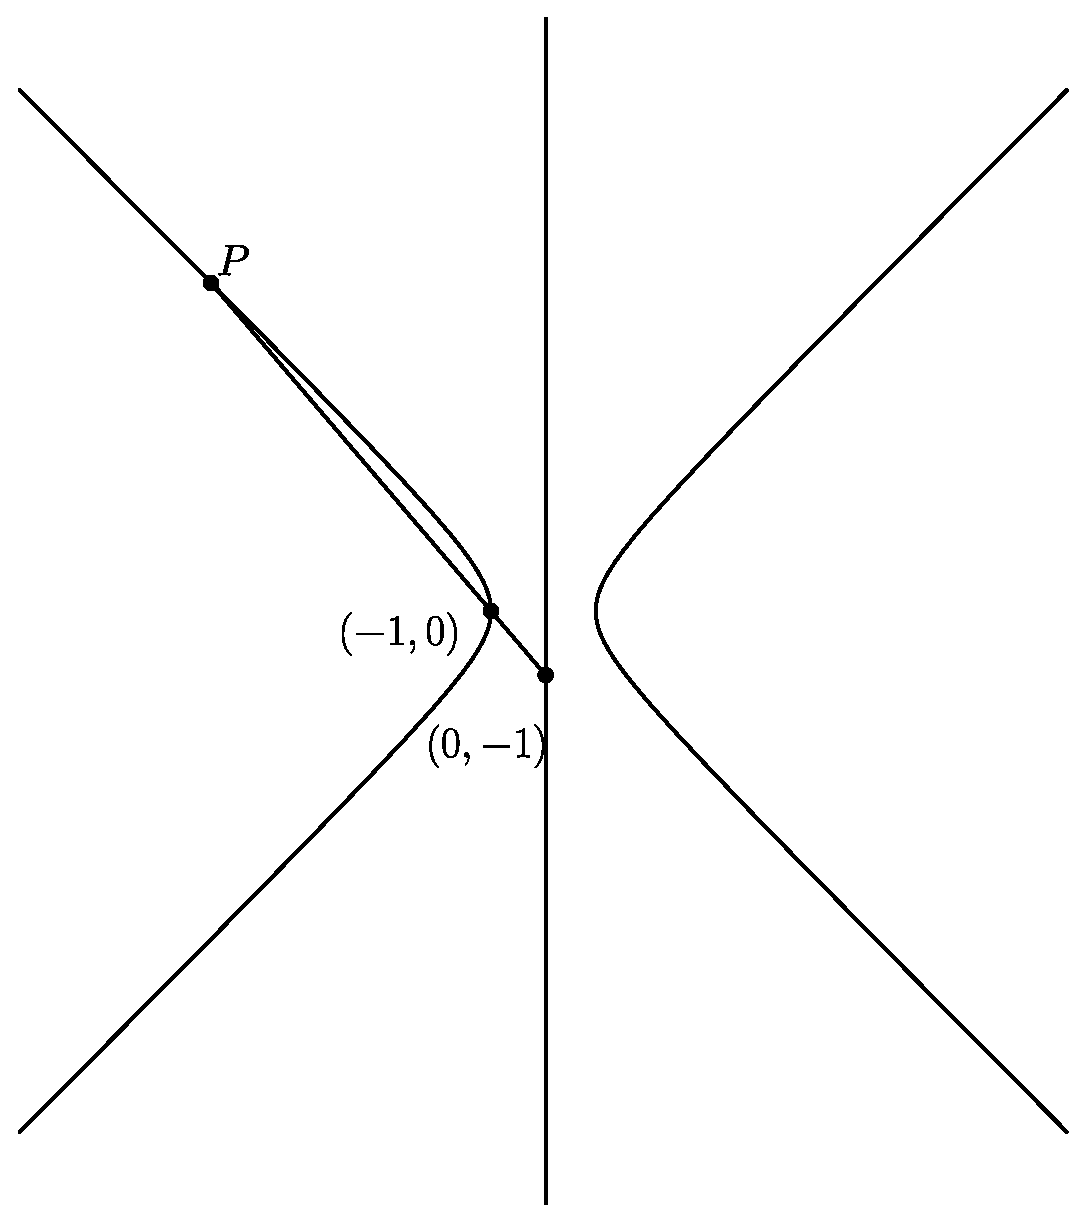
\includegraphics[scale=0.5]{Figures/Chapter1/rational_hyperbola.eps}
                 \caption{}
                 \label{figure_1.1}
             \end{figure}

         \item[(2)] Fermat's Last Theorem, states that the algebraic set
             $V:x^n+y^n=1$ has as $\Q$-rational points the set consisting of
             \begin{equation*}
                 V(\Q)=\begin{cases}
                        (1,0), (0,1),  \text{ if } n \equiv 0 \mod{2}   \\
                        (\pm{1},0), (0,\pm{1}) \text{ if } n \equiv 1 \mod{2}   \\
                     \end{cases}
             \end{equation*}

         \item[(3)] The algebraic set $V:y^2=x^3+17$ has many $\Q$-rational
             points, of which are
             \begin{align*}
                 (-2,3) &&  (5234,37866)    &&
                 \Big{(} \frac{137}{64},\frac{2651}{512} \Big{)}
             \end{align*}
    \end{enumerate}
\end{example}

\begin{definition}
    We call an affine algebraic set $V$ over a perfect field $k$ an \textbf{affine
    variety} if $I(V)$ is a prime ideal in $\bar{k}[x_1, \dots, x_n]$. We define
    the \textbf{affine coordinate ring} of $V$ to be the factor ring
    \begin{equation*}
        k[V]=\faktor{k[x_1, \dots,x_n]}{I(\faktor{V}{k})}
    \end{equation*}
We call the field of fractions of $k[V]$ the \textbf{function field} of $V$ over
 $k$ and denote it  $k(V)$. We similarly define $\bar{k}[V]$ to be
    \begin{equation*}
        \bar{k}[V]=\faktor{\bar{k}[x_1, \dots,x_n]}{I(\faktor{V}{\bar{k}})}
    \end{equation*}
    and $\bar{k}(V)$ to be the field of fractions of $\bar{k}(V)$.
\end{definition}

\begin{lemma}\label{1.1.4}
    The affine coordinate ring of a affine variety is an integral domain.
\end{lemma}
\begin{proof}
    Let $k$ be a perfect set, and  $V$ an affine variety over  $k$. By
    definition, we have that  $I(V)$ is a prime ideal in $\bar{k}[x_1,
    \dots,x_n]$; moreover, since $k$ is a field,  $k[x_1, \dots, x_n]$ is a
    commutative ring with identity. This means that $k[V]$ must be an integral
    domain (see proposition $13$; \cite{dummit-foote}).
\end{proof}

\begin{lemma}\label{1.1.5}
    Let $k$ be a perfect field, and $V$ an affine variety over $k$. Then  $k[V]$
    and $k(V)$ are subsets of $\bar{k}[V]$ and $\bar{k}(V)$ fixed by
    $\Gal{\faktor{\bar{k}}{k}}$.
\end{lemma}
\begin{proof}
    Excersice (see exercise $1.12$; \cite {silverman}).
\end{proof}

\begin{definition}
    Let $k$ be a perfect field. A  \textbf{transcendental base} of
    $\faktor{\bar{k}}{k}$ is a maximally algebraically independent subset of
    $\bar{k}$ over $k$. We define the \textbf{transcendence degree} of
    $\faktor{\bar{k}}{k}$ to be the cardinality of any given transcendental base
    of $\faktor{\bar{k}}{k}$, and denote it $\trdim{\faktor{k}{k}}$. We define
    the dimension on an affine variety over $k$ to be
    \begin{equation*}
        \dim{V}=\trdim{\faktor{\bar{k}(V)}{k}}
    \end{equation*}
\end{definition}

\begin{example}\label{example_1.2}
    $\dim{\A^n}=n$ since $\bar{k}(\A^n)=\bar{k}(x_1, \dots, x_n)$. Now, if $V
    \subseteq \A^n$ is a variety given by the polynomial equation
    \begin{equation*}
        f(x_1, \dots, x_n)=0
    \end{equation*}
    then $\dim{V}=n-1$.
\end{example}

\begin{definition}
    Let $V$ be an affine variety over $k$ such that $I(V)=(f_1, \dots ,f_m)$
    with $f_1, \dots f_m \in \bar{k}[x_1, \dots, x_n]$, and let $P \in V$. We
    call  $V$  \textbf{nonsingular} (or \textbf{smooth}) at $P$ if the  $m
    \times n$ matrix
\begin{equation*}
\begin{pmatrix}
\frac{\partial{f_1}}{\partial{x_1}} & \dots & \frac{\partial{f_1}}{\partial{x_n}}   \\
\vdots  &   \vdots  &   \vdots  \\
\frac{\partial{f_m}}{\partial{x_1}} & \dots & \frac{\partial{f_1}}{\partial{x_n}}   \\
\end{pmatrix}
\end{equation*}
    has rank $n-\dim{V}$. If $V$ is nonsingular at any point, then we call  $V$
    \textbf{nonsingular} (or \textbf{smooth}). We call $V$  \textbf{singular} if
    it is not nonsingular.
\end{definition}

\begin{lemma}\label{1.1.6}
    Let $V$ be an affine variety over a perfect field $k$, and $I(V)=(f)$ for
    some $f \in \bar{k}[x_1, \dots, x_n]$. Then $V$ is singular if, and only if
    \begin{equation*}
        \frac{\partial{f}}{\partial{x_1}}= \dots
        =\frac{\partial{f}}{\partial{x_1}}=0
    \end{equation*}
\end{lemma}
\begin{proof}
    We prove the contrapositve. Since $f$ is given by the polynomial equation
    $f(x_1, \dots ,x_n)=0$, then $\dim{V}=n-1$, so that if $V$ is nonsingular,
    then the  $1 \times n$ matrix
    \begin{equation*}
        \begin{pmatrix}
        \frac{\partial{f}}{\partial{x_1}} & \dots & \frac{\partial{f}}{\partial{x_n}} \\
        \end{pmatrix}
    \end{equation*}
    has rank $n-(n-1)=1$; in which case, we have for for all $1 \leq i \leq n$
    \begin{equation*}
        \frac{\partial{f}}{\partial{x_i}} \neq 0
    \end{equation*}
    The converse holds by similar reasoning.
\end{proof}

\begin{example}\label{example_1.3}
    Consider the affine varieties
    \begin{equation*}
        V_1:y^2=x^3+x \text{ and } V_2:y^2=x^3+x^2
    \end{equation*}
    Then a point of $V_1$, and $V_2$, respectively, is singular if
    \begin{equation*}
        2y=3x^2+1=0 \text{ and } 2y=3x^2+2x=0
    \end{equation*}
    Then $V_1$ is nonsingular, where as $V_2$ is singular at the point
    $P=(0,0)$. Letting $k=\Q$, and graphing the curves $y^2-x^3-x$ and
    $y^2-x^3-x^2$ in $\R^2$ in figure \ref{figure_1.2} shows us the singular and
    nonsingular points
    \begin{figure}[h]
        \centering
        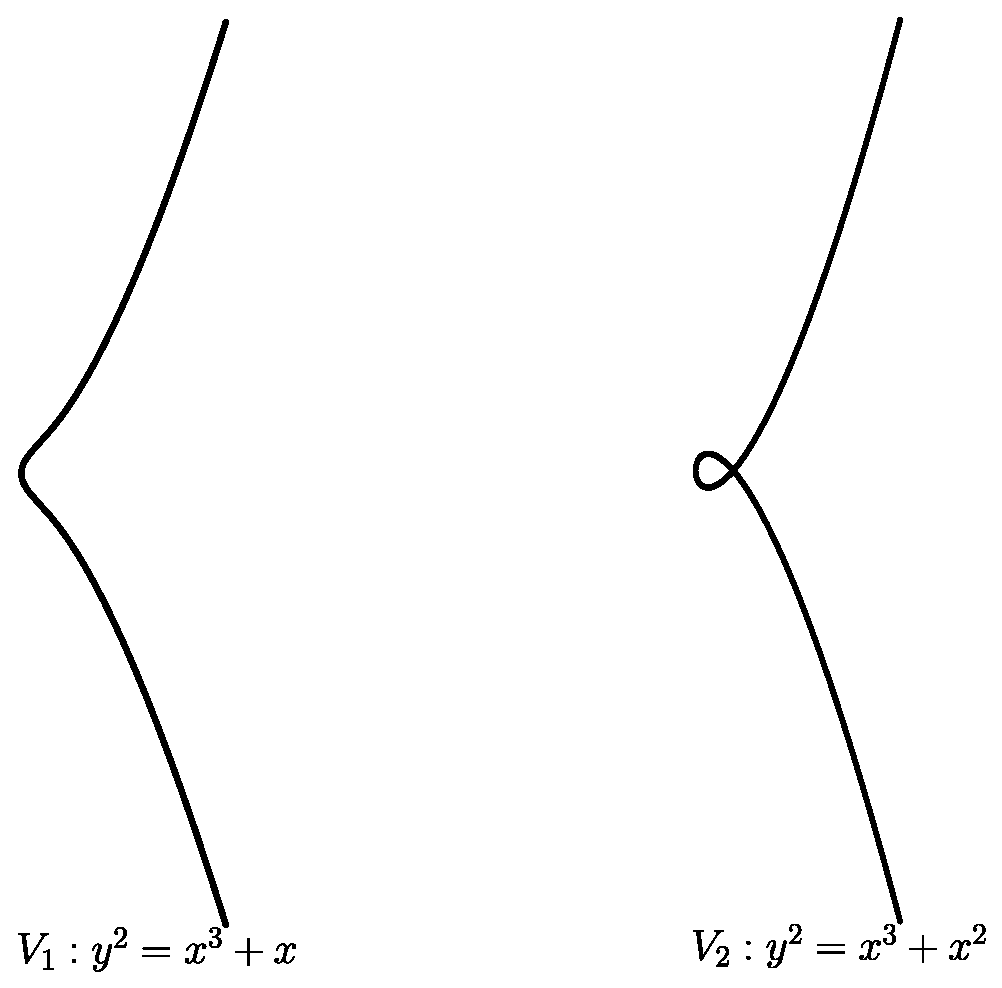
\includegraphics[scale=0.5]{Figures/Chapter1/nonsingular_singular.eps}
        \caption{}
        \label{figure_1.2}
    \end{figure}
\end{example}

\begin{lemma}\label{1.1.7}
    Let $V$ be an affine variety over a perfect field  $k$, and let  $P \in V$.
    Define $\mf_P$ of $\bar{k}[V]$ by
    \begin{equation*}
        \mf_P=\{f \in \bar{k}[x_1, \dots, x_n] : f(P)=0\}
    \end{equation*}
    Then $\mf_P$ is an idela of $\bar{k}[x_1, \dots, x_n]$, and $P$ is a
    nonsingular point of $V$ if, and only if
    \begin{equation*}
        \dim_{\bar{k}}{\faktor{\mf_P}{\mf_P^2}}=\dim{V}
    \end{equation*}
    where $\faktor{\mf_P}{\mf_P^2}$ is considered as a vector space.
\end{lemma}

\begin{example}\label{example_1.4}
    Consider again the varieties of example \ref{example_1.3}. Then $\mf_P$ is
    the ideal $\mf_P=(x,y)$ in $\bar{k}[x,y]$, and $\mf_P^2=(x^2,xy,y^2)$. Then
    we have
    \begin{equation*}
        x=y^2-x^3 \equiv 0 \mod{\mf_P^2}
    \end{equation*}
    so that $\faktor{\mf_P}{\mf_P^2}=(y)$ in the variety $V_1$. On the other
    hand, there is no nontrivial relation between $x$ and  $y$ in  $\mf_P^2$ for
     $V_2$, so that $\faktor{\mf_P}{\mf_P^2}$ must have $x$ and  $y$ as
     generators. Now,  $\dim{V_1}=\dim{V_2}=1$, implying, by lemma \ref{1.1.7}
     that $V_1$ is nonsingular and $V_2$ is singular.
\end{example}

\begin{definition}
    Let $V$ be an affine variety over a perfect field $k$. We define the
    \textbf{local ring} of $V$ at  $P$, denoted $\bar{k}[V]_P$ to be the
    localization of $\bar{k}[V]$ at $\mf_P$. That is
    \begin{equation*}
        \bar{k}[V]_P=\Big{\{} F \in \bar{k}(V) : f=\frac{f}{g}, f,g \in
            \bar{k}[x_1, \dots, x_n] \text{ and } g(P) \neq 0 \Big{\}}
    \end{equation*}
\end{definition}
